\documentclass[10pt,a4paper]{report}
\usepackage[utf8]{inputenc}
\usepackage{amsmath}
\usepackage{amsfonts}
\usepackage{amssymb}
\usepackage{amsthm}
\usepackage{natbib}
\usepackage{titlesec}
\usepackage{tikz}
\usepackage[ruled,linesnumbered]{algorithm2e}
\SetKw{KwBy}{by}

\setcounter{secnumdepth}{4}

\usepackage[mathscr]{euscript}
\usepackage{tikz}

\newcommand{\Cross}{\mathbin{\tikz [x=2.5ex,y=2.5ex,line width=.10ex] \draw (0,0) -- (1,1) (0,1) -- (1,0);}}

\newcommand*{\N}{\mathbb{N}}
\newcommand*{\R}{\mathbb{R}}
\DeclareMathOperator*{\argminA}{arg\,min}

\newcommand{\mathDef}{\overset{\textit{def}}{=}}

\usepackage{hyperref}
\hypersetup{
    colorlinks=true, %set true if you want colored links
    linktoc=all,     %set to all if you want both sections and subsections linked
    linkcolor=black,  %choose some color if you want links to stand out
}

\theoremstyle{definition}

\newtheorem{definition}{Definition}[section]
\newtheorem*{remark}{Remark}

\begin{document}
	
\tableofcontents
\newpage


\begin{equation}
	\begin{array} {lllrr} 
		\text{min} & \displaystyle\sum_{n = 1}^N \sum_{k = 1}^K \sum_{x \in C} g(x)^{f_k^i} Y_x^{f_k^i} \\\\
		& \displaystyle\sum_{n = 1}^N \sum_{k = 1}^K \sum_{x \in C} T(x)^{f_k^i} Y_x^{f_k^i} & \leq &  D_{\textbf{F}} \\
		& \displaystyle\sum_{n = 1}^N \sum_{k = 1}^K \sum_{x \in C} Y_x^{f_k^i} & = & 1 \\\\
		& Y_x^{f_k^i} \in \lbrace 0, 1 \rbrace &&
	\end{array}
\end{equation}


\begin{equation}
	\begin{array} {lllrr} 
		\text{min} & \displaystyle\sum_{\pi \in \Pi} \sum_{n = 1}^N \sum_{k = 1}^K \sum_{x \in C} g(x)^{f_k^i} Y_{(\pi, x)}^{f_k^i} \\\\
		& \displaystyle\sum_{n = 1}^N \sum_{k = 1}^K \sum_{x \in C} T(x)^{f_k^i} Y_x^{f_k^i} & \leq &  D_{\textbf{F}} \\
		& \displaystyle\sum_{\pi \in \Pi} \sum_{n = 1}^N \sum_{k = 1}^K \sum_{x \in C} Y_{(\pi, x)}^{f_k^i} & = & 1 \\\\
		& Y_{(\pi, x)}^{f_k^i} \in \lbrace 0, 1 \rbrace &&
	\end{array}
\end{equation}


\newpage

\section{Serverless Computing Paradigm}

In serverless computing platforms, computation is done by so-called \textit{function instances} which are completely managed by the serverless computing platform provider and act as tiny servers that can be invoked based on events forwarded by end-users \cite{PMSCP}.

Serverless computing platforms handle almost every aspect of the system administration tasks needed to deploy a workload on the cloud, providing a new simplified programming model according to which developers can focus on the business aspects of their applications only \cite{COSE}.

Moreover, the paradigm lowers the cost of deploying applications too, adopting a so-called “\textit{pay as you go}” pricing model, by charging for execution time rather than for allocated resources \cite{COSE}.


\subsection{Serverless Function}

A \textit{serverless function} represents a stateless, event-driven, self-contained unit of computation implementing a business functionality.

Although a serverless function generally represents a unit of executable code, submitted to FaaS platforms by developers using one or a combination of the programming languages supported by FaaS providers, a serverless function can be any cloud services eventually necessary to business logic, like cloud storage, message queue services, pub/sub messaging service etc.

When it represents executable code, developers can specify several configuration parameters, like timeout, memory size or CPU power \cite{COSE}.

A serverless function can be triggered through events or HTTP requests following which the FaaS provider executes it in a containerized environment, like container, virtual machine or even processes, using the specified configuration.

\subsection{Serverless Application}

In serverless paradigm, the most basic scenario is to invoke a single function through a HTTP request; however, if you want to built more complex applications, constructing so-called \textit{serverless application}, serverless functions must be connected and appropriately coordinated.

Formally, we define a serverless application as a stateless and event-driven software system made up of a serverless functions set hosted on one or more FaaS platforms and combined together by a so-called \textit{coordinator} (or \textit{orchestrator}).

Generally, the coordinator is a broker needed to implement the business logic of any application: it chains together serverless function, handles events among functions and triggers them in the correct order according to the business logic defined by developers. 

Most public cloud providers for serverless computing have introduced platforms to define and coordinate serverless function in order to built serverless application, like AWS Step Functions which combines multiple Lambda functions and other serverless services offered by AWS into responsive serverless applications

Although FaaS platforms continuously advance the support for serverless applications, existing solutions are dominated by a few large-scale providers resulting in mostly non-portable FaaS solutions 

and provider lock-in

occurs when transitioning data, products, or services to another vendor's platform is difficult and costly, making customers more dependent (locked-in) on a single cloud storage solution.

FC languages and runtime systems are still in their
infancy with numerous drawbacks. Current commercial and open
source offerings of FC systems are dominated by a few large-
scale providers who offer their own platforms, 

As FaaS platforms take over operational responsibilities,
besides uploading the source code of functions, users have
limited control over resources on FaaS platforms. Taking
AWS Lambda as an example, the amount of allocated mem-
ory during execution and the concurrency level are only op-
tions for tuning the performance of functions. The amount
of allocated memory is between 128 MB and 3,008 MB
in 64MB increments [13]. Previous researches have proven
that computational power and network throughput are in
proportion to the amount of allocated memory, and disk
performance also increases with larger memory size due
to less contention [14], [15]. By reserving and provisioning
more instances to host functions, high concurrency level can
decrease fluctuations in the function performance incurred
by cold starts (container initialization provisioning delay if
no warm instance is available) and reduce the number of
throttles under very heavy request loads



\subsection{fdsfsd}




\begin{itemize}
	\item 
\end{itemize}

\subsection{title}


Serverless computing has given a much-needed agility to
developers, abstracted away the management and maintenance
of physical resources, and provided them with a relatively
small set of configuration parameters: memory and CPU.
While relatively simpler, configuring the “best” values for
these parameters while minimizing cost and meeting perfor-
mance and delay constraints poses a new set of challenges.
This is due to several factors that can significantly affect the
running time of serverless functions.


the run-time of these serverless
functions decreases with the increase of memory size allocated
to the function. However, the marginal improvement in the
run-time decreases as the memory increases.

This behavior
is because the pricing model as exposed by the cloud providers
is tightly coupled with the amount of resources specified
to execute the serverless function (c.f. Figure 1a), and the
dependency between memory and CPU resource allocation –
AWS Lambda allocates CPU power


a model for each executable belonging to a given choreography.



This helps developers decide if a developed
workload would comply with their QoS agreements, and if
not, how much performance improvement they would need
to do so. The performance improvement decided could be
achieved either by improving the design, quality of code, or
by simply resizing the resource allocated to each instance,
which is usually set by changing the allocated memory.


A cold start 

Cold/Warm start: as defined in previous work [3], [8],
[10], we refer to cold start request when the request goes
through the process of launching a new function instance.
For the platform, this could include launching a new virtual
machine, deploying a new function, or creating a new
instance on an existing virtual machine, which introduces an
overhead to the response time experienced by users. In case
the platform has an instance in the idle state when a new
request arrives, it will reuse the existing function instance
instead of spinning up a new one. This is commonly known
as a warm start request. Cold starts could be orders of
magnitude longer than warm starts for some applications.
Thus, too many cold starts could impact the application’s
responsiveness and user experience [3].



his equation gives the probability of a request being
rejected (blocked) by the warm pool, assuming there are m
warm servers. If m is less than the maximum concurrency
level, the request blocked by the warm pool causes a cold
start. If the warm pool has reached the maximum concur-
rency level, any request rejected by the warm pool will be
rejected by the platform.



\section{Orchestrator Model}

\subsection{Resource owner}

A \textit{resource owner}, henceforward denoted with $R$, represents an entity capable of \textit{creating}, \textit{modifying} and \textit{authorizing} access to several resources of our system.

\newpage

\chapter{Specification Mode}
\section{Serverless Choreography}

In this section we will introduce the notion of \textit{serverless choreography}, a very important \textit{resource} adopted to model and implement both serverless functions and serverless applications.

Informally, the notion of serverless choreography has been derived from that of a control-flow graph; as known, the latter describes, using graph notation, all paths that might be traversed through a serverless application during its execution. Similarly, a serverless choreography describes calling relationships between serverless functions which can be combined using several types of control-flow connectors.

\subsection{Preliminary Definitions}

Before to define what we mean for serverless choreography, is necessary to introduce some very useful notations.

Let $n \in \N$ and $G = (\Phi,E)$ a directed graph, where:

\begin{itemize}
	\item $\Phi$ is a finite set of vertices, such that $|\Phi| = n$;
	\item  $E \subseteq \Phi \times \Phi $ is a finite set of ordered pairs of vertices $e_{ij} = \left( \phi_i, \phi_j \right)$, where $\phi_i \in \Phi$ to $\phi_j \in \Phi$ for any $i,j \in \N \cap \left[ 1, n \right]$. Any ordered pair of vertices is also called directed edge;
\end{itemize}

Then, we will adopt following notations:

\begin{itemize}
	\item A \textit{path} of $G$ is defined as a finite sequence of distinct vertices and edges. We will denote a path by $\pi$ which formally can be represented as follows:
	
	\begin{equation}
		\pi = \phi_1 e_1 \phi_2 e_2 \ldots e_{n-2}\phi_{n-1} e_{n-1} \phi_n
	\end{equation}
	
	where:
	
	\begin{itemize}
		\item $\phi_i \in \Phi$, for all $i \in \N \cap \left[ 1, n \right]$
		\item $e_i = \left( \phi_i, \phi_{i+1} \right) \in E$, for all $i \in \N \cap \left[ 1, n-1 \right]$
	\end{itemize}
	
	\item Let $\phi_i,\phi_j \in \Phi$ for any $i,j \in \N \cap \left[ 1, n \right]$, the set denoted by $\Pi(\phi_i, \phi_j)$ identifies all possible paths starting from vertex $\phi_i$ and ending at vertex $\phi_j$.
	
	\item For any $u \in \N \cap \left[ 1, n \right]$, the set $out(\phi_u)$ ($in(\phi_u)$) denotes all edges starting (ending) from (to) vertex $\phi_u$, while the set $succ(\phi_u)$ ($pred(\phi_u)$) includes all direct successor (predecessors) vertices of $\phi_u$. Formally:
	
	\begin{eqnarray}\label{outDef}
		out(\phi_u) & \mathDef & \left\lbrace (\phi_u, \phi) \in E, \quad \forall \phi \in \Phi  \right\rbrace \\
		in(\phi_u) & \mathDef & \left\lbrace (\phi, \phi_u) \in E, \quad \forall \phi \in \Phi  \right\rbrace \\
		succ(\phi_u) & \mathDef & \left\lbrace \phi \in \Phi \mid (\phi_u, \phi) \in out(\phi_u)  \right\rbrace \\
		pred(\phi_u) & \mathDef & \left\lbrace \phi \in \Phi \mid (\phi, \phi_u) \in in(\phi_u)  \right\rbrace 
	\end{eqnarray}
	
	
\end{itemize}

\subsection{Definition}

According to the serverless paradigm, the execution of a serverless application starts with a particular function, which we will call \textit{entry point}, while any other serverless functions, belonging to the application, will be invoked subsequently according to specified business logic defined by developers; as we will see shortly, the latter can be naturally modeled by a weighted directed graph.

Clearly, the execution of a serverless application ends when the execution of the last function of the application ends; that ending function will be call as \textit{end point}. We assume that the entry point is unique.

Let $n \in \N \setminus \left\lbrace 0 \right\rbrace $ and $R$ a resource owner.

A \textit{serverless choreography} owned by $R$, or simply \textit{choreography} of $R$, is a resource represented by a weighted directed graph denoted as follows:

\begin{equation}
	\mathcal{C}_R \mathDef (\Phi,E)
\end{equation}

where:

\begin{itemize}
	\item $|\Phi| = n$;
	
	\item Each vertex $\phi \in \Phi$ is called \textit{abstract serverless function} and represents a computational unit; we will describe more in detail what we mean by abstract serverless function shortly;
	
	\item Let $i,j \in \N \cap \left[ 1, n \right]$ and $\phi_i, \phi_j \in \Phi$, any directed edge $e_{ij} = \left( \phi_i, \phi_j \right) \in E$ represents the calling relationship between two abstract serverless function which depends on the business logic defined by $R$. 
	
	In our context, any directed edge $\left( \phi_i, \phi_j \right) \in E$ states that the abstract serverless function $\phi_j$ \textit{can} be called by $\phi_i$;
	
	\item Let $i,j \in \N \cap \left[ 1, n \right]$, the number $p_{ij} \in \R \cap \left[ 0, 1 \right]$ is the weight assigned to the edge $\left(\phi_i, \phi_j \right) \in E$, where: 
	
	\begin{itemize}
		
		\item The number $p_{ij}$ represents the so-called \textit{transition probability} from $\phi_i$ to $\phi_j$, that is the probability of invoking $\phi_j$ after finishing the execution of $\phi_i$;
		
		\item We will use a function $P : \Phi \times \Phi \to \left[ 0, 1 \right]$, called \textit{transition probability function}, such that $P\left(\phi_i, \phi_j \right) = p_{ij}$. When $P\left(\phi_i, \phi_j \right) = 0$, it implies that the directed edge $\left( \phi_i, \phi_j \right) \notin E$, therefore $\phi_i$ cannot invoke $\phi_j$;
		
		\item For any path $\pi = \phi_1 e_1 \ldots e_{n-1} \phi_n$ of $\mathcal{C}_R$, we define \textit{transition probability of the path $\pi$} the following quantity:
		
		\begin{equation}
			TPP(\pi) = \prod_{i = 1}^{n-1} P\left(\phi_i, \phi_{i+1} \right)
		\end{equation}
		
	\end{itemize}
	
	\item $\Phi$ contains only one serverless abstract function, denoted by $\phi_{entry}$, acting as the entry point and at least one acting as the end point, which is denoted, instead, by $\phi_{end}$. Formally, we define aforementioned vertices as follows: 
	
	\begin{equation}
		\begin{array}{lcll}
			\phi \in \Phi & \text{ is the entry point of } \mathcal{C_R} & \Leftrightarrow & in(\phi) = \emptyset \\
			\phi \in \Phi & \text{ is the end point of } \mathcal{C_R} & \Leftrightarrow & out(\phi) = \emptyset
		\end{array}
	\end{equation}
	
	Then, following conditions must be hold:
	
	\begin{eqnarray}
		\exists !  \phi \in \Phi &\mid & in(\phi) = \emptyset \label{cond1} \\
		\exists   \phi \in \Phi & \mid & out(\phi) = \emptyset \label{cond2}
	\end{eqnarray}
	
	Finally, we will also use the notation $\alpha(\mathcal{C}_R)$ to denote the entry point $\phi_{entry}$ of a choreography $\mathcal{C}_R$. Conversely, we will adopt the notation $\omega(\mathcal{C}_R)$ to denote the set of all end points of $\mathcal{C}_R$
	
	\item Must be hold the condition according to which the transition probabilities of all paths between the entry point and	the end point of $\mathcal{C}_R$ sum up to $1$. Formally:
	
	\begin{equation}\label{cond3}
		\sum_{\phi_{end} \in \omega(\mathcal{C}_R)} \Big( \sum_{\pi \in \Pi(\phi_{entry}, \phi_{end})} TPP(\pi) \Big) = 1
	\end{equation}
	
	In other words, above conditions guarantees that any execution starting from $\phi_{entry}$ will terminate.
	
	\item A function, denoted by $D : \Phi \times \Phi \to \left[ 0, \infty \right)$, represents a delay function according to which $D\left(\phi_i, \phi_j \right)$ identifies the delay from $\phi_i$ to $\phi_j$ due to network delay or orchestration task;  
	
\end{itemize} 

A choreography $\mathcal{C}_R$ can be uniquely identified by an ordered pair $(a, b)$, where $a$ is the name of the resource owner $R$, while $b$ is the function choreography name.

Clearly, we say that choreography models a serverless function when $|\Phi| = 1$ and $|E| = 0$; conversely, it models a serverless function application when $|\Phi| > 1$ and $|E| > 0$.

From now, a choreography $\mathcal{C}_R$ will be briefly denoted by $\mathcal{C}$ when no confusion can arise about the resource owner $R$.

\subsubsection{Abstract Serverless Function}

Supposing that a choreography $\mathcal{C} = (\Phi,E)$ is given.

As said previously, any $\phi \in \Phi$ is called \textit{abstract serverless function}, or simply \textit{abstract function}, that is a \textit{resource} representing a computational unit required by business logic provided by developers.

According to our model, there are two types of abstract functions implementations:

\begin{itemize}
	
	\item $\phi$ is called \textit{serverless executable functions}, or simply \textit{executable function}, when $\phi$ contains executable code; therefore, in that case, we said that an executable function models a serverless function.
	
	$\mathscr{F_E}$ is defined as the set containing all executable function of $\mathcal{C}$ and it is formally defined as follows:
	
	\begin{equation}
		\mathscr{F_E} \mathDef \left\lbrace \phi \in \Phi \mid \phi \text{ is a serverless executable function }\right\rbrace 
	\end{equation}
	
	However, multiple different implementations of a given executable function can be provided by developers which, although they must be semantically and logically equivalent, may eventually expose different performance or cost behavior. 
	
	For any $\phi \in \mathscr{F_E}$, we will use $\textbf{F}_{\phi}$ notation to represent the so-called \textit{implementation-set} of $\phi$, that is the set containing any concrete implementation, denoted as $f_{\phi}$, of $\phi$.
	
	Later, we will explain how our framework is able to pick, for all $\phi \in \mathscr{F_E}$, exactly one $f_{\phi} \in \textbf{F}_{\phi}$ whose properties allow us to meet user-specified QoS objective.
	
	\item $\phi$ is called \textit{serverless orchestration functions}, or simply \textit{orchestration functions}, when $\phi$ contains the so-called \textit{orchestration code}. 
	
	According to our model, orchestration code represents the logic required to chain together any components of an application, handling events and triggering executable functions in the correct order according to the business logic. In other words, orchestration code is used to manage the control-flow of any application; later we will describe how it is possible.
	
	$\mathscr{F_O}$ is defined as the set containing all orchestration functions of $\mathcal{C}$ and it is formally defined as follows:
	
	\begin{equation}
		\mathscr{F_O} \mathDef \left\lbrace \phi \in \Phi \mid \phi \text{ is a serverless orchestration function }\right\rbrace 
	\end{equation}
	
\end{itemize}

Clearly, based on above definitions, we can say: 

\begin{eqnarray}
	\mathscr{F_E} \cap \mathscr{F_O} & = & \emptyset \\
	\mathscr{F_E} \cup \mathscr{F_O} & = & \Phi \\
	|\mathscr{F_E}| + |\mathscr{F_O}| &=& |\Phi| 
\end{eqnarray}

Any abstract function $\phi$ is uniquely identified by an ordered pair $(a, b)$, where:
\begin{itemize}
	\item $a$ represents the identifier of the choreography $\mathcal{C}$;
	\item $b$ is the name of the abstract serverless function $\phi$;
\end{itemize}

\subsubsection{Executability condition}

Let $\mathcal{C} = (\Phi,E)$ a choreography.

Obviously, in order to effectively start the execution of a choreography, is required that, for each executable function $\phi \in \mathscr{F_E}$, \textit{at least one} concrete implementation $f_{\phi}$ exists.

Formally, we said that a choreography is \textit{executable} when: 

\begin{eqnarray}
	\label{eqn:SchedulabilityConditionOne}
	\mathcal{C} \text{ is executable } & \Leftrightarrow & |\textbf{F}_{\phi}| \geq 1 \qquad \forall \phi \in \mathscr{F_E}
\end{eqnarray}

We will only deal with executable choreographies. Moreover, for all $\phi \in \mathscr{F_E}$, we always assume that all $f_{\phi} \in \textbf{F}_{\phi}$ are already deployed on one or more FaaS platform by developers.

\subsubsection{Serverless Sub-choreography}

Let $\mathcal{C} = (\Phi,E)$ a choreography. 

The weighted directed sub-graph of $\mathcal{C}$ defined as follows:

\begin{equation}
	\mathcal{C}^* \mathDef (\Phi^*,E^*) \qquad \text{ where } \Phi^* \subseteq \Phi \wedge E^* \subseteq E
\end{equation}

is called \textit{serverless sub-choreography} of $\mathcal{C}$, or simply \textit{sub-choreography} of $\mathcal{C}$, when the conditions \ref{cond1}, \ref{cond2} and \ref{cond3} are hold.

\subsubsection{Basic Serverless Choreography}\label{BasicDefinition}

Suppose to have a choreography $\mathcal{C} = (\Phi,E)$ satisfying following conditions:

\begin{eqnarray}
	|\mathscr{F_O}| = 0 \label{cond21} \\
	|\omega(\mathcal{C})| = 1 \label{cond22}
\end{eqnarray}

We said that any choreography $\mathcal{C}$, satisfying the conditions \ref{cond21} and \ref{cond22}, represents a \textit{basic serverless choreography}, or simply a \textit{basic choreography}.

\section{Serverless Choreography Configuration}

Given a choreography $\mathcal{C} = (\Phi,E)$, the basic goal of our framework is to determine a so-called \textit{serverless choreography configuration}, called also \textit{choreography configuration} or, simply, \textit{configuration}, allowing us to meet user-specified QoS objectives.

Informally, a configuration specifies which concrete function will be use for all executable function inside a choreography, specifying several parameters, like memory size or CPU power.

\subsection{Executable Function Configuration}

In this section, we will explain the concept of \textit{executable function configuration}. 

Let $\phi \in \mathscr{F_E}$ an executable function and $\textbf{F}_{\phi}$ the corresponding implementation-set.

Formally, an \textit{executable function configuration} $x_{\phi}$ for the executable function $\phi$ is a two-dimensional vector defined as follows:

\begin{equation}
	x_{\phi} = (f_{\phi},m) \in f_{\phi} \times \textbf{M}_{f_{\phi}} \subseteq \textbf{F}_{\phi} \times \N
\end{equation}

where:

\begin{itemize}
	\item $f_{\phi} \in \textbf{F}_{\phi}$  denotes a particular concrete function implementing the executable function $\phi$.
	\item $m \in \textbf{M}_{f_{\phi}}$ represents the allocated memory size during the execution of $f_{\phi}$, where $\textbf{M}_{f_{\phi}} \subseteq \N$ is the set holding all available memory size configurations allowed by provider where the concrete function $f_{\phi}$ is executed.
\end{itemize}

\subsection{Serverless Choreography Configuration}

Let $n,k \in \N \setminus \left\lbrace 0 \right\rbrace$ and a choreography $\mathcal{C} = (\Phi,E)$ such that $|\Phi| = n$ and $|\mathscr{F_E}| = k$ where $k \leq n$.

Formally, a \textit{serverless choreography configuration} $\textbf{X}_{\mathcal{C}}$ for the choreography $\mathcal{C}$ is a vector such that:

\begin{eqnarray}
	\textbf{X}_{\mathcal{C}} & \mathDef & \left\lbrace x_{\phi_{1}}, \ldots, x_{\phi_{k}} \right\rbrace \nonumber \\ 
	& \in & \left\{  \left\{ \bigcup_{j=1}^{|\textbf{F}_{\phi_{1}}|} f_{\phi_{1_j}} \times \textbf{M}_{f_{\phi_{1_j}}} \right\} \times \ldots \times \left\{ \bigcup_{j=1}^{|\textbf{F}_{\phi_{k}}|} f_{\phi_{k_j}} \times \textbf{M}_{f_{\phi_{k_j}}} \right\} \right\}  \nonumber \\
	& = & \Cross_{i = 1}^k \left\{ \bigcup_{j=1}^{|\textbf{F}_{\phi_{i}}|} f_{\phi_{i_j}} \times \textbf{M}_{f_{\phi_{i_j}}} \right\} \nonumber \\
	& \subseteq & \Cross_{i = 1}^k \left\{ \textbf{F}_{\phi_{i}} \times \mathbb{N} \right\}
\end{eqnarray}

where:

\begin{itemize}
	\item $x_{\phi_{i}}$ represents the executable function configuration for the executable function $\phi_{i}$, for some  $i \in \N \cap \left[ 1, k \right]$.
	
	\item $f_{\phi_{i_j}}$ represent the $j$-th concrete function implementing the executable function $\phi_{i}$, for some  $i \in \N \cap \left[ 1, k \right]$ and $j \in \N \cap \left[ 1, |\textbf{F}_{\phi_{i}}| \right]$.
	
	\item $\textbf{M}_{f_{\phi_{i_j}}} \subseteq \N$ denotes the set containing all available memory size options, allowed by provider, during the execution of the concrete function $f_{\phi_{i_j}}$, for some $i \in \N \cap \left[ 1, k \right]$ and $j \in \N \cap \left[ 1, |\textbf{F}_{\phi_{i}}| \right]$
\end{itemize}

\section{Executable Function Performance}

In order to select an appropriate serverless choreography configuration able to effectively deliver and guarantee the QoS level required by our users, we need to evaluate the performance of any executable function inside a choreography when a particular concrete function is chosen to implement it. 

\subsection{Concurrency level}

Any FaaS platform imposes a limitation on the number of serverless function instance runnable at the same time; this limit is generally known as \textit{concurrency level} or \textit{concurrency limits}. 

Clearly, this kind of limitation is needed to assure enough resources for all users using the services provided by FaaS platform. However, despite all FaaS providers impose aforementioned limitation, these restriction are applied differently.

Informally speaking, there are two type of concurrency limit models:

\begin{description}
	\item[Global (Per-Account) Concurrency Model] according to which invocation threshold is shared by all serverless functions belonging to a given resource owner. 
	
	For example, in $2022$, this approach is adopted both by AWS Lambda and IBM Cloud Functions, which do not allow more than $1000$ serverless concrete function in running state at the same time.
	
	\item[Local (Per-Function) Concurrency Model] where, opposed to global concurrency model, any invocation threshold is applied only on individual concrete functions. 
	
	This approach is adopted by Google Cloud Functions although there are reports stating that, despite there is no explicitly mentioned global concurrency limit, a kind of global concurrency limit, varying between $1000$ and $2000$, is observed.
	
\end{description}

\subsection{Platform provider modelling}

In order to formalize the notion of concurrency limit, explaining its role inside the way according to which serverless executable function performance are computed, is necessary to explain how FaaS platform providers had been modeled.

From our model point of view, any FaaS platform provider can acting as a ``\textit{set}'' of $M/G/K(t)_{\textbf{C}_{max}}/K(t)_{\textbf{C}_{max}}$ queueing systems, where:

\begin{itemize}
	
	\item $\textbf{C}_{max} \in \N$ represents the \textit{maximum value of queue concurrency limit}, that is the maximum number of function instances being in running state simultaneously at time $t$ inside that queue. 
	
	Please note that $\textbf{C}_{max}$ not necessary coincide with global concurrency limit because it can represents a local concurrency limit too.
	
	\item At time $t \geq 0$, there are $K(t)$ function instances that can each process one request and the system has capacity for $K(t)$ invocation requests in total. 
	
	In other words, the number of function instance, and consequently the capacity of system, can change over time. 
	
	At any time $t$, following condition must be hold:
	
	\begin{equation}
		0 \leq K(t) \leq {C}_{\textbf{max}}
	\end{equation}
	
	\item No queue is involved, therefore any incoming request at time $t$, which sees all $K(t)$ function instances busy and $K(t) = \textbf{C}_{\textbf{max}}$, is considered dropped.
	
	\item No priority is considered among incoming request.
	
	\item Service times have a general distribution while a Poisson arrival process is assumed.
\end{itemize} 

Please note that, according to our model, any FaaS platform can host several $M/G/K(t)_{\textbf{C}_{max}}/K(t)_{\textbf{C}_{max}}$ queueing systems, many of which can belong to an unique resource owner.  

\subsection{Serverless concrete function swarms}

To complete the formalization of our model, is necessary to introduce another very important concept.

Let $l \in \N$, $R$ a resource owner, $P$ a serverless computing platform provider and $\Omega_{P_R}$ the set of all concrete serverless functions hosted on $P$ and belonging to $R$. 

A \textit{serverless concrete function swarms} is any set $\omega_{P_{R_l}} \subseteq \Omega_{P_R}$ containing all concrete functions belonging to $R$ that share the same limit $l$ in term of the max number of serverless function instance runnable at the same time by the corresponding platform provider $P$. 
	
That limit can be called \textit{server-less function swarm's concurrency limit}, or simply, \textit{concurrency limit}.
	
Is very important to make clear that only at most $l$ concrete functions belonging to $\omega_{P_{R_l}}$ can be executed simultaneously by $P$. Clearly, the value of $l$ depends on the concurrency model by $P$ and this kind of formalization make our model compatible with both approaches described previously. Formally:

\begin{itemize}
	
	\item If $P$ imposed a \textit{per-function} limit, then $|\omega_{P_{R_l}}| = 1$, that is, $\omega_{P_{R_l}}$ contains only one function and $l$ will represent the provider's per-function limit. 
	
	In that case, there is a $M/G/K(t)_{l}/K(t)_{l}$ queuing system for each concrete function in $\Omega_{P_R}$, every of which will serve all invocation request regarding only one concrete function in $\omega_{P_{R_l}}$.
	
	In other words, there are $|\omega_{P_{R_l}}|$ different queues.
	
	\item If $P$ imposed a \textit{per-account} limit, then $\omega_{P_{R_l}} = \Omega_{P_R}$, that is the swarm includes all concrete serverless concrete function deployed on $P$ by $R$ and $l$ represents the provider's global concurrency limit. 
	
	In that case, there is only one $M/G/K(t)_{l}/K(t)_{l}$ queuing system serving all invocation request regarding any concrete function in $\omega_{P_{R_l}}$.

\end{itemize}

\subsection{Executable function state}

Similarly to previous studies, a function instance can be in one of the following states: 

\begin{description}
	
	\item[Initialization State] which happens when the infrastructure is spinning up new function instances which are needed to handle incoming requests. 
	
	Generally, depending on the approach adopted by the FaaS provider, during this state is needed to set up new virtual machines, unikernels, containers, or even, processes, in order to be able to process new requests.
	
	A function instance will remain in the initializing state until it is able to handle incoming requests, entering into idle state. The time spent in this state is not billed. 
	
	\item[Idle State] After the fulfillment of all initialization task or when the processing of a previously received invocation request is over, the serverless platform keeps the instances in idle state, keeping the function instance able to handle future invocation request faster, since no initialization task is needed to be performed.
	
	FaaS platform provider keeps a function instance in idle state for a limited amount of time. The user is not charged for an instance that is in the idle state.
	
	\item[Running State] When an invocation request is submitted to an function instance, the latter goes into the running state, according to which aforementioned request is parsed and processed.
	
	Clearly, the time spent in the running state is billed by the provider.
		
\end{description}

\subsection{Start/Cold start}

\begin{description}
	\item[Cold start] If the warm pool is busy, that is there are no serverless function instances in idle state able to serve an newly incoming request, latter will trigger the launching of a new function instance, which will be added to the warm pool. This event is called \textit{cold start}.
	
	From the FaaS provider point of view, this operation requires to start either a new virtual	machine or a new container; in any case, regardless of the method adopted, a cold start introduces a very important overhead to the response time experienced by users. 
	
	\item[Warm start] When there is at least one serverless function instance in idle state, the FaaS platform reuses it to serve the incoming request without launching a new one. This is called \textit{warm start}.
\end{description}  

A very important aspect is that cold starts could be orders of magnitude longer than warm starts for some applications; therefore, too many cold starts could impact the application’s responsiveness and user experience.

Precisely, let $\gamma \in \N$, $\omega_{P_{R(\gamma)}}$ a swarm where $\gamma$ is the maximum concurrency level of the swarm. Finally, let $M/G/K(t)_{\gamma}/K(t)_{\gamma}$ a queuing system, that is the swarm queue of $\omega_{P_{R(\gamma)}}$. 

When a new invocation request, regarding any function belonging $\omega_{P_{R(\gamma)}}$, arrives on the FaaS platform $P$, one of the following events can occur:

\begin{itemize}
	\item If at time $t$ is verified that $K(t) < \gamma$, that is the number of function instances into the warm pool is less than the maximum concurrency level, only one of following events can occur:
	
	\begin{itemize}
		\item if $|\mathcal{R}(t)| = K(t)$, that is there, the request will be blocked by the system causing a cold start.
		
		\item if $|\mathcal{R}(t)| < K(t)$ a warm start will occur and $\mathcal{R}(t)$ is increased by one.
	\end{itemize}
	
	\item If at time $t$ is true that $K(t) = \gamma$, that is the warm pool size reaches the maximum concurrency level admitted by provider $P$, and $|S(t)| = \gamma$, namely every there is no function instance in idle state, any further request will be rejected by the platform and therefore dropped by our controller.
	
\end{itemize}

\subsubsection{Cold start probability}

As known, the rejection of a request by the warm pool triggers a cold start, which, subsequently, adds a new function instance to the warm pool in order to handle received request. 

In order to fully describe how our framework works, we have to know the probability according to which a request is rejected by the warm pool; in other words, we must to compute the \textit{cold start probability}. 

Let $k \in N$ the size of the warm pool, that is the number of existing function instances currently active on the provider.

Formally, the cold start probability $\textbf{P}_{C_R}$ is the probability that an arrival finds all $k$ function instances of the warm pool busy. Using Erlang-B formula, aforementioned probability can be calculated as follows:

\begin{equation}
	\displaystyle \textbf{P}_{C}(t) = \dfrac{\dfrac{\rho(t)^k}{k!}}{\displaystyle\sum_{j=0}^k \dfrac{\rho(t)^j}{j!}}
\end{equation}

where:

\begin{itemize}
	
	\item $\displaystyle \rho(t) = \frac{\lambda(t)}{\mu_{w}}$ represents system utilization or load of the pool at time $t$ where:
	
	\begin{itemize}
		
		\item $\lambda(t)$ represents the \textit{average arrival rate} at time $t$, that is the  rate at which serverless compound functions execution requests arrive to our system.
		
		Since we assume that arrival rate varies during the day, $\lambda(t)$ is estimate over multiple time intervals spent observing our system.
		
		Precisely, at time $t$, let $n \in \N$ the number of request arrived during last second 
		
		\begin{equation}
			\lambda(t) \mathDef
			\begin{cases}
				0 & \text{if}\ t = 0\\ 
				\alpha \cdot X + (1 - \alpha) \cdot \lambda(t-1) & \text{if}\ t > 0\\
				
			\end{cases}\,.
		\end{equation}
		
		\item $\mu_{w} = E[S_w]$ represents the \textit{warm start average service rate}, that is the rate at which executions requests are served when a warm start is occurred, while $E[S_w]$ is the \textit{warm start average time}, which is the average time required to complete aforementioned request.
		
	\end{itemize}
	
\end{itemize}


\section{Concrete function performance}

At this point, we can define some useful functions:

\begin{itemize}	
	\item $C_{\textbf{F}_{\phi}} : \textbf{F}_{\phi} \times \N \to \left[ 0, \infty \right)$ is the \textit{cost function} for any serverless functions belonging to the implementation-set $\textbf{F}_{\phi}$.
	
	Precisely, for all $f_{\phi} \in \textbf{F}_{\phi}$ and $m \in \N$, $C_{\textbf{F}_{\phi}}(f_{\phi}, m)$ returns the \textit{average cost} paid by developers to execute $f_{\phi}$ using an allocated memory size equal to $m$.
	
	
	\item $RT_{\textbf{F}_{\phi}} : \textbf{F}_{\phi} \times \N \to \left[ 0, \infty \right)$ is a \textit{delay function} for any serverless functions belonging to the implementation-set $\textbf{F}_{\phi}$.
	
	For all $f_{\phi} \in \textbf{F}_{\phi}$ and $m \in \N$, $RT_{\textbf{F}_{\phi}}(f_{\phi}, m)$ returns the \textit{average response time} when $f_{\phi}$ is invoked with memory size equal to $m$;
\end{itemize}






\section{The problem of cold starts}

In order to find a suitable serverless choreography configuration capable to satisfy QoS imposed by end users, we must find a way to decide  





\subsection{Metrics}

Let $\mathcal{C} = (\Phi,E)$ a basic choreography as defined in section \ref{BasicDefinition}.



Suppose to have a path $\pi = \phi_1 e_1 \phi_2 e_2 \ldots e_{n-2}\phi_{n-1} e_{n-1} \phi_n$ and a choreography configuration $\textbf{X}$ for $\mathcal{S}$. 

We can define the \textit{response time} of $\pi$ given $\textbf{X}$ as follows:

\begin{equation}
	RT_P(\pi, \textbf{X}) = \sum_{i = 1}^n \left( RT_{\phi_i} (X(i) \right)  + \sum_{i = 1}^{n-1} D(\phi_i,\phi_{i+1})
\end{equation}

Similarly, we define the cost of $\pi$ given $\textbf{X}$ as follows:

\begin{equation}
	C_P(\pi, \textbf{X}) = \sum_{\substack{1\le i\le n\\ \phi_i \in \mathscr{F_E}}} N(\phi_i) \cdot C_{\textbf{F}_{\phi_i}} (X(i))
\end{equation}


Then the response time and the cost of the choreography $\mathcal{S}$ a follows:

\begin{eqnarray}
	RT_C(\mathcal{S}, \textbf{X}) & = & \sum_{\pi \in \Pi(\phi_{entry}, \phi_{end})} TPP(\pi) \cdot RT_{P}(\pi, \textbf{X}) \\
	C_C(\mathcal{S}, \textbf{X}) & = & \sum_{\pi \in \Pi(\phi_{entry}, \phi_{end})} TPP(\pi) \cdot C_{P}(\pi, \textbf{X}) 
\end{eqnarray}



\section{Serverless Choreography Structures}

Let $\mathcal{C} = (\Phi,E)$ a serverless choreography. 

Formally


Supposing to have a serverless choreography $\mathcal{S} = (\Phi,E)$, we call \textit{structure} any sub-choreography $\mathcal{S}^*= (\Phi^*,E^*)$ whose entry point and the end point are, respectively, an opening and a closing orchestration functions of the same type. Formally:

\begin{equation}
	S^* \text{ is a structure } \Leftrightarrow \left\{ \begin{array}{rlll}
		\phi_{entry}^* & \in \mathscr{F_O^*} & \wedge & \mathscr{T}(\phi_{entry}^*) = \tau_{\alpha} \\ 
		\phi_{end}^* & \in \mathscr{F_O^*} & \wedge & \mathscr{T}(\phi_{end}^*) = \tau_{\omega}
	\end{array} \right.
\end{equation}

The most important aspect is that every structure can be viewed as a set of sub-choreographies of $\mathcal{S}^*$. Formally, suppose that $\Lambda = (A,B)$ is a graph such that:

\begin{equation}
	\begin{array}{lll}
		A & \mathDef & \Phi^* \setminus \left\lbrace \phi_{entry}^*,\phi_{end}^* \right\rbrace   \\
		B & \mathDef & E^* \setminus \left( out\left(\phi_{entry}^*\right) \cup in\left(\phi_{end}^*\right) \right)
	\end{array}
\end{equation}

Let $c \in \N$ and suppose that $c$ is the number of connected components of the graph $\Lambda$.

We denote by $\Theta_{\mathcal{S}^*}$ as the set containing all connected components of $\Lambda$ every of which is considered as a sub-choreography of $\mathcal{S}^*$. Formally:

\begin{equation}
	\begin{array}{c}
		\Theta_{\mathcal{S}^*} \mathDef \left\lbrace \theta_i, \ldots ,\theta_c \right\rbrace \\\\
		\text{ where } \\\\
		
		\theta_i \mathDef (\Phi^{**}_i, E^{**}_i) \text{ is a sub-choreography of } \mathcal{S}^* \\
		\Phi^{**}_i \subset \Phi^{*} \wedge E^{**}_i \subset E^{*} \qquad \forall i \in \left[ 1, c \right] \\
	\end{array}
\end{equation} 

\subsubsection{Parallel}

A structure $\mathcal{P} = (\Phi,E,\Theta)$ is called \textit{parallel structure} when:

\begin{equation}
	TPP(\pi) = 1 \qquad \forall \pi \in \Pi(\phi_{start}, \phi_{end})
\end{equation}



\begin{figure}[h!]
	\centering
	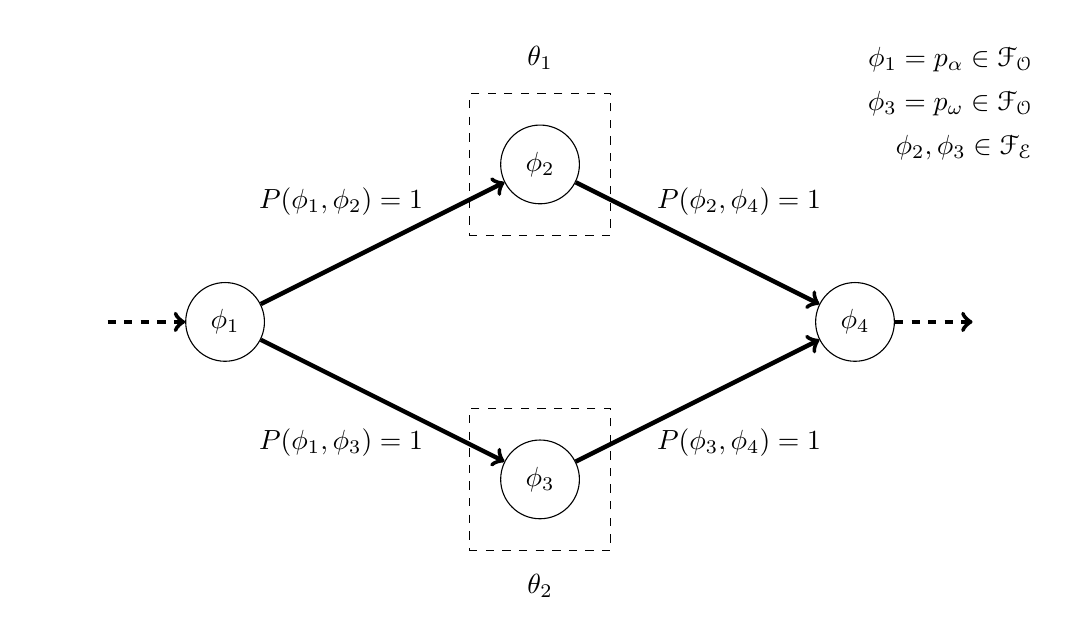
\begin{tikzpicture}
		
	
		\node[circle,draw=white,minimum width = 1cm] 
		(start) at (-2,0) {};
	
		\node[circle, draw, minimum width = 1cm]        					   
		(ParStartNode) at (0,0) {$\phi_1$};
		
	
		\node[circle, draw, minimum width = 1cm]        					   
		(ParNode1) at (4,2) {$\phi_2$};
		\node[circle, draw, minimum width = 1cm]       					   
		(ParNode2) at (4,-2) {$\phi_3$};
		
		\node[circle, draw, minimum width = 1cm]        					   
		(ParEndNode) at (8,0) {$\phi_4$};
			
		\node[circle,draw=white,minimum width = 1cm] 
		(end) at (10,0) {};
		
		
		\draw[ultra thick,->] (ParStartNode) edge node[xshift=-15 ,yshift=15]{$P(\phi_1,\phi_2) = 1$} (ParNode1);
		\draw[ultra thick,->] (ParStartNode) edge node[xshift=-15 ,yshift=-15]{$P(\phi_1,\phi_3) = 1$} (ParNode2);
		
		\draw[ultra thick,->] (ParNode1) edge node[xshift=15 ,yshift=15]{$P(\phi_2,\phi_4) = 1$} (ParEndNode);
		\draw[ultra thick,->] (ParNode2) edge node[xshift=15 ,yshift=-15]{$P(\phi_3,\phi_4) = 1$} (ParEndNode);
		
		\draw[dashed,ultra thick, ->] (start) -- (ParStartNode);
		\draw[dashed,ultra thick, ->] (ParEndNode) -- (end);
		
		% Frames
		
		\node[rectangle, draw, dashed, minimum width =1.8cm, minimum height=1.8cm] (sub1) at (4,2) {};
		\node[circle,above of=sub1, yshift=10] (label1) {$\theta_1$};
		
		\node[rectangle, draw, dashed, minimum width =1.8cm, minimum height=1.8cm] (sub2) at (4,-2) {};
		\node[circle,below of=sub2, yshift=-10] (label2) {$\theta_2$};
		
		%legend
		
		\matrix [below left] at (current bounding box.north east) {
			\node [] {$\phi_1 = p_{\alpha} \in \mathscr{F_O}$}; \\
			\node [] {$\phi_3 = p_{\omega} \in \mathscr{F_O}$}; \\
			\node [] {$\phi_2, \phi_3 \in \mathscr{F_E}$}; \\
		};
		
		
\end{tikzpicture}
\caption{Parallel structure in the serverless workflow.}
\end{figure}



Let $n \in \N$, supposing that $|\Theta| = n$, the response time of a parallel structure is the longest response time of all sub-choreographies $\theta_i \in \Theta$ for all $i \in \left[ 1, n \right]$, while its cost is equal to the sum their costs of execution. Formally, being $\textbf{X}$ a configuration of  $\mathcal{P}$:

\begin{equation}
	RT_{parallel}(\mathcal{P}, \textbf{X}) = max \left\lbrace RT_C(\mathcal{\theta}, \textbf{X}) \mid \theta \in \Theta \right\rbrace 
\end{equation}

\begin{equation}
	C_{parallel}(\mathcal{P}, \textbf{X}) = \sum_{\theta \in \Theta} C_C(\theta, \textbf{X})
\end{equation}



\subsubsection{Branch/Switch}

Let $\mathcal{B} = (\Phi,E,\Theta)$ a structure and suppose that $\alpha(\mathcal{B}) = \phi_{entry}$ and $\omega(\mathcal{B}) = \phi_{end}$. 

$\mathcal{B}$ is called \textit{branch structure} when following conditions are hold:

\begin{eqnarray}
	TPP(\pi) \neq 1  & \quad \forall \pi \in \Pi(\phi_{entry}, \phi_{end}) \\
	|\Theta| = n  & n \in \left\lbrace 1,2 \right\rbrace 
\end{eqnarray}

\begin{figure}[h!]
	\centering
	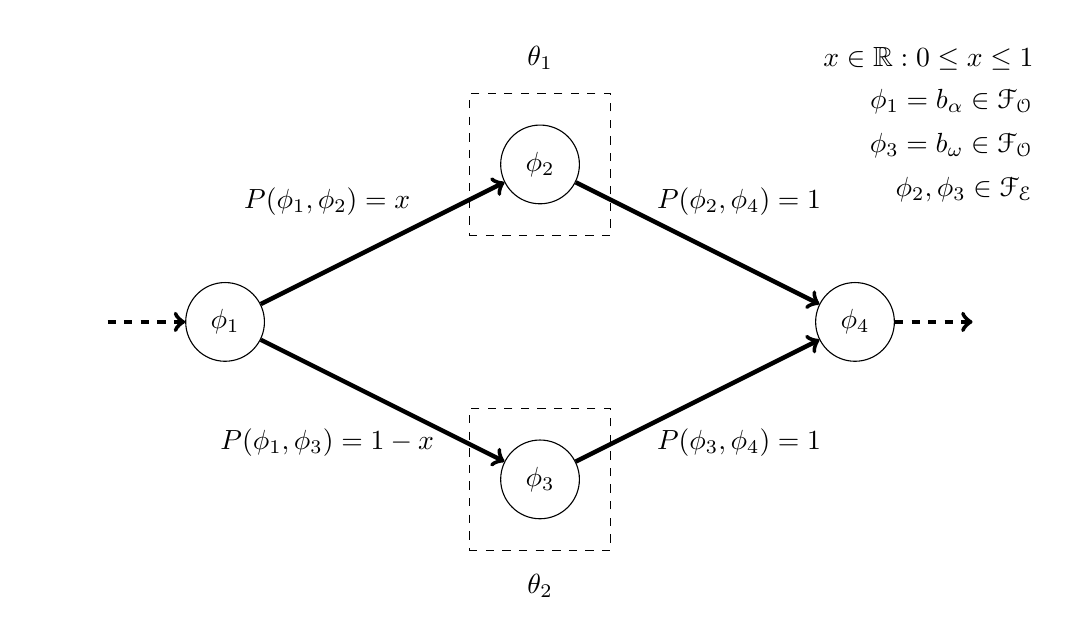
\begin{tikzpicture}
		
		
		\node[circle,draw=white,minimum width = 1cm] 
		(start) at (-2,0) {};
		
		\node[circle, draw, minimum width = 1cm]        					   
		(ParStartNode) at (0,0) {$\phi_1$};
		
		
		\node[circle, draw, minimum width = 1cm]        					   
		(ParNode1) at (4,2) {$\phi_2$};
		\node[circle, draw, minimum width = 1cm]       					   
		(ParNode2) at (4,-2) {$\phi_3$};
		
		\node[circle, draw, minimum width = 1cm]        					   
		(ParEndNode) at (8,0) {$\phi_4$};
		
		\node[circle,draw=white,minimum width = 1cm] 
		(end) at (10,0) {};
		
		
		\draw[ultra thick,->] (ParStartNode) edge node[xshift=-20 ,yshift=15]{$P(\phi_1,\phi_2) = x$} (ParNode1);
		\draw[ultra thick,->] (ParStartNode) edge node[xshift=-20 ,yshift=-15]{$P(\phi_1,\phi_3) = 1-x$} (ParNode2);
		
		\draw[ultra thick,->] (ParNode1) edge node[xshift=15 ,yshift=15]{$P(\phi_2,\phi_4) = 1$} (ParEndNode);
		\draw[ultra thick,->] (ParNode2) edge node[xshift=15 ,yshift=-15]{$P(\phi_3,\phi_4) = 1$} (ParEndNode);
		
		\draw[dashed,ultra thick, ->] (start) -- (ParStartNode);
		\draw[dashed,ultra thick, ->] (ParEndNode) -- (end);
		
		% Frames
		
		\node[rectangle, draw, dashed, minimum width =1.8cm, minimum height=1.8cm] (sub1) at (4,2) {};
		\node[circle,above of=sub1, yshift=10] (label1) {$\theta_1$};
		
		\node[rectangle, draw, dashed, minimum width =1.8cm, minimum height=1.8cm] (sub2) at (4,-2) {};
		\node[circle,below of=sub2, yshift=-10] (label2) {$\theta_2$};
		
		%legend
		
		\matrix [below left] at (current bounding box.north east) {
			\node [] {$x \in \mathbb{R} : 0 \leq x \leq 1$}; \\
			\node [] {$\phi_1 = b_{\alpha} \in \mathscr{F_O}$}; \\
			\node [] {$\phi_3 = b_{\omega} \in \mathscr{F_O}$}; \\
			\node [] {$\phi_2,\phi_3 \in \mathscr{F_E}$}; \\
		};
		
		
	\end{tikzpicture}
	\caption{Branch/Switch structure in the serverless workflow.}
\end{figure}

Let all $\theta_i \in \Theta$ sub-choreographies of $\mathcal{B}$, for all $i \in \left\lbrace 1,2 \right\rbrace $. Then the response time and the cost of a branch structure can be defined as follows:

\begin{equation}
	RT_{branch}(\mathcal{B}, \textbf{X}) = \sum_{i = 1}^n P(\phi_{entry}, \alpha(\theta_i)) RT_C(\theta_i, \textbf{X})
\end{equation}

\begin{equation}
	C_{branch}(\mathcal{B}, \textbf{X}) = \sum_{i = 1}^n C_C(\phi_{entry}, \alpha(\theta_i)) C_C(\theta_i, \textbf{X})
\end{equation}

Finally, according to our model, $\mathcal{B}$ is called \textit{switch structure} when $|\Theta| > 2$.

\subsubsection{Loop}

Let $\mathcal{L} = (\Phi,E,\Theta)$ a structure and suppose that $\alpha(\mathcal{L}) = \phi_{entry}$ and $\omega(\mathcal{L}) = \phi_{end}$. 

If $|\Theta| = 1$ and $(\phi_{end}, \phi_{entry}) \in E$, denoting by $\theta$ the unique sub-choreography of $\mathcal{L}$, $\mathcal{L}$ will be called \textit{loop structure} when following conditions are hold:

\begin{eqnarray}
	P(\phi_{start}, \alpha(\theta)) = 1 \\
	P(\phi_{end}, \phi_{entry}) \neq 0 \\
	P(\phi_{end}, \phi_{entry}) + \sum_{\phi \in succ(\phi_{end})} P(\phi_{end}, \phi) = 1
\end{eqnarray}

\begin{figure}[h!]
	\centering
	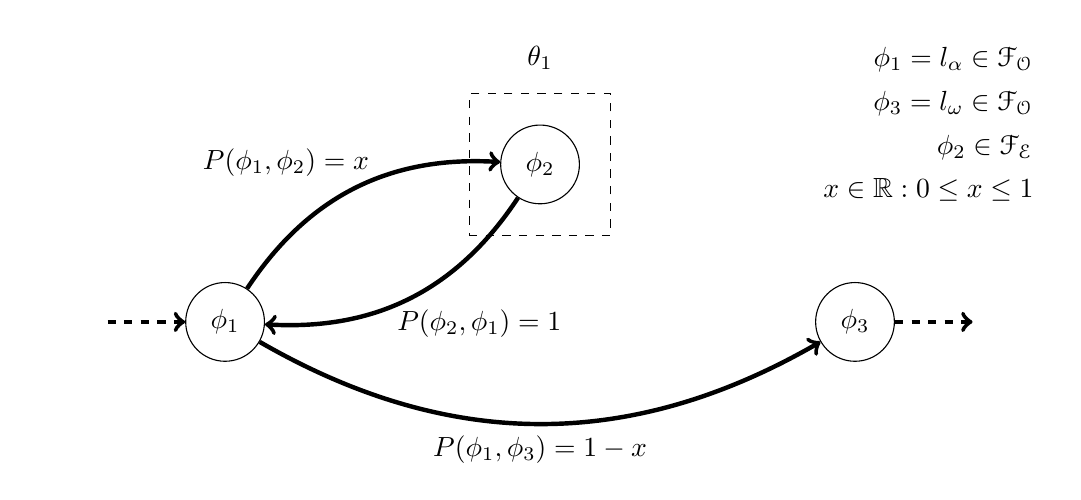
\begin{tikzpicture}
		
		
		\node[circle,draw=white,minimum width = 1cm] 
		(start) at (-2,0) {};
		
		\node[circle, draw, minimum width = 1cm]        					   
		(ParStartNode) at (0,0) {$\phi_1$};
		
	
		\node[circle, draw, minimum width = 1cm]        					   
		(ParNode1) at (4,2) {$\phi_2$};
	
		
		\node[circle, draw, minimum width = 1cm]        					   
		(ParEndNode) at (8,0) {$\phi_3$};
		
	
		
		\node[circle,draw=white,minimum width = 1cm] 
		(end) at (10,0) {};
		
		
		\draw[bend left,above, ultra thick,->] (ParStartNode) edge node[xshift=-25]{$P(\phi_1,\phi_2) = x$} (ParNode1);
		
		\draw[bend left,below, ultra thick,->] (ParNode1) edge node[xshift=25]{$P(\phi_2,\phi_1) = 1$} (ParStartNode);
		
		\draw[bend right,below, ultra thick,->] (ParStartNode) edge node[]{$P(\phi_1,\phi_3) = 1 - x$} (ParEndNode);
		
		
		
		\draw[dashed,ultra thick, ->] (start) -- (ParStartNode);
		\draw[dashed,ultra thick, ->] (ParEndNode) -- (end);
		
		% Frames
		
		\node[rectangle, draw, dashed, minimum width =1.8cm, minimum height=1.8cm] (sub1) at (4,2) {};
		\node[circle,above of=sub1, yshift=10] (label1) {$\theta_1$};
	
		%legend
	
		\matrix [below left] at (current bounding box.north east) {
			\node [] {$\phi_1 = l_{\alpha} \in \mathscr{F_O}$}; \\
			\node [] {$\phi_3 = l_{\omega} \in \mathscr{F_O}$}; \\
			\node [] {$\phi_2 \in \mathscr{F_E}$}; \\
			\node [] {$x \in \mathbb{R} : 0 \leq x \leq 1$}; \\
		};
		
	\end{tikzpicture}
	\caption{Parallel structure in the serverless workflow.}
\end{figure}



In order to compute the mean response time and the mean cost of a loop structure, we need to know $EI(\mathcal{L})$, that is the expected value of the number of iterations of $\mathcal{L}$.

We know that geometric distribution gives the probability that the first occurrence of success requires $k \in \N$ independent trials, each with success probability $p$ and failure probability $q = 1 - p$. In our case, if the our success corresponds to event "we will not execute the loop body", we know that success probability $p$ is given by:

\begin{equation}
	p = 1 - P(\phi_{end}, \phi_{entry})
\end{equation}

Then:

\begin{eqnarray}
	P(EI(\mathcal{L}) = k) & = & \Big[  1 - P(\phi_{end}, \phi_{entry}) \Big] \cdot \bigg[  P(\phi_{end}, \phi_{entry}) \bigg] ^{k-1} \\
	& = & pq^{k-1}
\end{eqnarray}

\begin{eqnarray}
	E[X] & = & \sum_{k = 1}^\infty (k-1) pq^{k-1} \nonumber \\
	& = & p \sum_{k = 0}^\infty kq^{k} \nonumber \\
	& = & p \cdot \frac{q}{(1-q)^2} \nonumber \\
	& = & \dfrac{q}{p} \nonumber \\
	& = & \dfrac{P(\phi_{end}, \phi_{entry})}{1 - P(\phi_{end}, \phi_{entry})} 
\end{eqnarray}

Then the response time and the cost of a loop structure can be defined as follows:

\begin{equation}
	RT_{loop}(\mathcal{L}, \textbf{X}) = E[I_{\mathcal{L}}] \cdot RT_C(\theta, \textbf{X})
\end{equation}

\begin{equation}
	C_{loop}(\mathcal{L}, \textbf{X}) = E[I_{\mathcal{L}}] \cdot C_C(\theta, \textbf{X})
\end{equation}




\section{Optimization}


\subsection{Performance Modeling}






We define the utility function as follows:

\begin{equation}
	F(\textbf{x}) \mathDef w_{RT} \cdot \dfrac{RT_{max} - RT(\textbf{x})}{RT_{max} - RT_{min}} + w_{C} \cdot \dfrac{C_{max} - C(\textbf{x})}{C_{max} - C_{min}}
\end{equation}

where $w_{RT}, w_{C} \geq 0$, $w_{RT} + w_{C} = 1$, are weights for the different QoS attributes, while $RT_{max}$ ($RT_{min}$) and $C_{max}$ ($C_{min}$) denote, respectively, the maximum (minimum) value for the overall expected response time and cost.


Following formulation is based on the enumeration of all possible choreography configurations, that is of all combinations of executable function configuration of a given choreography.

For the sake of conciseness, in the following we use following notation: 

p to define both a pattern and its index, and $\Omega$ to define both the set of patterns and the
set of patterns indices.



\begin{equation}
	\begin{array} {rll} 
		\displaystyle max & \displaystyle \sum_{\omega = 1}^{|\Omega|} x_{\omega} F(\textbf{X}_{\omega}) \\\\
		
		\text{subject to} & \displaystyle \sum_{\omega = 1}^{|\Omega|} x_{\omega} C(\textbf{X}_{\omega}) \leq C_{user} \\\\
		
		& \displaystyle \sum_{\omega = 1}^{|\Omega|} x_{\omega} RT(\textbf{X}_{\omega}) \leq RT_{user} \\\\ 
		
		& \displaystyle \sum_{\omega = 1}^{|\Omega|} x_{\omega} = 1 & \\\\
		
		
		& x_{\omega} \in \lbrace 0, 1 \rbrace & \qquad \forall \omega \in \N \cap [1,|\Omega|]
	\end{array}
\end{equation}

Above formulation is based on the enumeration of all possible choreography configuration.






\newpage
\subsection{Multi-dimensional Multi-choice Knapsack Problem}

Let $\mathcal{C} = (\Phi,E)$ a choreography. 

For the sake of consciousness, we will use $\mathcal{\widetilde{P}}$ to denote the set containing all parallel structures of $\mathcal{C}$, while $\mathcal{\widetilde{P}}_i$ is used to refer to $i$-th parallel structure of $\mathcal{\widetilde{P}}$, where $i \in \N \cap \left[1;|\mathcal{\widetilde{P}}| \right]$.

Let's define $\Delta_{\mathcal{\widetilde{P}}_{i_j}}$ the set containing all executable functions $\phi \in \mathscr{F_E}$ belonging to the $j$-th sub-choreography of the parallel structure $\mathcal{\widetilde{P}}_i$. Formally:

\begin{equation}
	\Delta_{\mathcal{\widetilde{P}}_{i_j}} \mathDef \left\{ \phi \in \mathscr{F_E} \cap \mathscr{F_E}(\theta_j) \text{ where } \theta_j \in  \right\} 
\end{equation}

We 

\begin{eqnarray}
	\chi & \mathDef & \left\lbrace \Delta_{\mathcal{\widetilde{P}}_{1}}, \ldots, \Delta_{\mathcal{\widetilde{P}}_{n}} \right\rbrace \nonumber \\ 
	& \in & \left\{  \left\{ \bigcup_{j=1}^{|\mathcal{\widetilde{P}}_i|} \Delta_{\mathcal{\widetilde{P}}_{1_j}} \right\} \times \ldots \times \left\{ \bigcup_{j=1}^{|\mathcal{\widetilde{P}}_n|} \Delta_{\mathcal{\widetilde{P}}_{n_j}} \right\} \right\}  \nonumber \\
	& = & \Cross_{i = 1}^n  \left\{ \bigcup_{j=1}^{|\mathcal{\widetilde{P}}_i|} \Delta_{\mathcal{\widetilde{P}}_{1_j}} \right\}  \nonumber \\
\end{eqnarray}




\begin{equation}
	\begin{array} {rll} 
		\displaystyle max & \displaystyle \sum_{i = 1}^{|\mathscr{F_E}|}  \sum_{j = 1}^{|\textbf{F}_{\phi_{i}} \times \N|} x_{\phi_{i_{j}}} p_{\phi_{i_{j}}} \\\\
		
		\text{subject to} & \displaystyle \sum_{i = 1}^{|\mathscr{F_E}|}  \sum_{j = 1}^{|\textbf{F}_{\phi_{i}} \times \N|} x_{\phi_{i_{j}}} c_{\phi_{i_{j}}} \leq C_{user} \\\\
		
	    
		
		
		& \displaystyle \sum_{\phi_i \in \mathscr{F_E} \cap \mathscr{F_E}(\mathcal{\widetilde{P}})}  \sum_{j = 1}^{|\textbf{F}_{\phi_{i}} \times \N|} x_{\phi_{i_{j}}} t_{\phi_{i_{j}}} + \sum_{\phi_i \in \chi}  \sum_{j = 1}^{|\textbf{F}_{\phi_{i}} \times \N|} x_{\phi_{i_{j}}} t_{\phi_{i_{j}}} \leq RT_{user} & \qquad \forall \xi \in \Xi \\\\    
		 
		
		& \displaystyle \sum_{j = 1}^{|\textbf{F}_{\phi_{i}} \times \N|} x_{\phi_{i_{j}}} = 1 & \qquad \forall i \in \N \cap \left[ 1, |\mathscr{F_E}| \right] \\\\
		
		& x_{\phi_{i_{j}}} \in \lbrace 0, 1 \rbrace & \qquad \forall i \in \N \cap \left[ 1, |\mathscr{F_E}| \right] \wedge \forall j \in \N \cap [1,|\textbf{F}_{\phi_{i}} \times \N|]
	\end{array}
\end{equation}


The MMKP is an NP-hard in the strong sense [2]. It is not
always possible to find a feasible solution in a reasonable
computing time especially for big instances. Since exact
methods are reserved for limited scale problem, heuristic
approaches are needed for solving it. 



Let $\mathcal{C} = (\Phi,E)$ a serverless choreography, $x_{\phi_{i_{j}}} = (f_j, m_j) $ an executable function configuration for the executable function $\phi_i \in \mathscr{F_E}(\mathcal{C})$, for some $i \in \N \cap [1,|\mathscr{F_E}(\mathcal{C})|]$ and $j \in \N \cap [1,|\textbf{F}_{\phi_{i}} \times \N|]$. 

Let's define $\widehat{\theta_k}^{(\phi_i)} = {\theta^{(\phi_i)}_1, \ldots, \theta^{(\phi_i)}_n}$  as the sequence of all sub-choreographies of $\mathcal{C}$ such that:

\begin{equation}
	\phi_i \in \mathscr{F_E}(\theta^{(\phi_i)}_1)
\end{equation}

\begin{equation}
	\theta^{(\phi_i)}_n = \mathcal{C}
\end{equation}

\begin{equation}
	\theta^{(\phi_i)}_k \text{ is a sub-choreography of } \theta^{(\phi_i)}_{k+1} \qquad \forall k \in \left[1;n-1\right]
\end{equation}

At this point, we can define $E[I_{\phi_i}]$, that is the expected value of the number of invocations of the executable function $\phi_i$, as follows.

\begin{equation}	
	E[I_{\phi_i}] \mathDef \left\{
	\begin{array}{lcr}
		1 & \text{\textit{if}} & n = 1 \\ 
		\displaystyle \prod_{k = 2}^n E[I_{\theta_{k-1}^{(\phi_i)}}] & \text{\textit{if}} & n \geq 2 \\
	\end{array} \right.
\end{equation}

For some $k \in \N \cap \left[1;n-1\right]$, we will use $P_{exe}^C(\theta^{(\phi_i)}_k)$ notation to refer to the probability to execute the abstract function entry point $\alpha(\theta^{(\phi_i)}_k)$ of the choreography $\theta^{(\phi_i)}_k$, when the abstract function $pred(\alpha(\theta^{(\phi_i)}_k))$ is invoked. That probability can be computed as follows:

\begin{equation}	
	P_{exe}^C(\theta^{(\phi_i)}_k) \mathDef \left\{
	\begin{array}{lcr}
		1 & \text{\textit{if}} & n = 1 \\ 
	    P \bigg(  pred\Big( \alpha(\theta^{(\phi_i)}_{k}) \Big), \alpha(\theta^{(\phi_i)}_{k}) \bigg) & \text{\textit{if}} & n \geq 2 \\
	\end{array} \right.
\end{equation}


Finally, we define $P_{exe}^{F}(\theta, \phi)$ as the probability to execute the executable function $\phi \in \mathscr{F_E}(\theta)$ when the abstract function $\alpha(\theta)$ is invoked. We can compute this probability using following formula:

\begin{equation}
	P_{exe}^{F}(\theta, \phi) \mathDef \prod_{\phi_k \in \mathscr{F_O}(\theta) \cap preds(\phi)} (1 - P_{exit}(\phi_k))
\end{equation}

Defining:

\begin{equation}
	\Gamma_{\phi_{i_{j}}} \mathDef E[I_{\phi_i}] \prod_{k = 2}^{n}  P_{exe}^C(\theta^{(\phi_i)}_{k-1}) \cdot P_{exe}^{F}(\theta^{(\phi_i)}_{k}, pred(\alpha(\theta^{(\phi_i)}_{k-1})))
\end{equation}

we can compute resource requirements $c_{\phi_{i_{j}}}$ and $t_{\phi_{i_{j}}}$ in the following ways:


\begin{eqnarray}
	c_{\phi_{i_{j}}} & \mathDef & \left\{ 
	\begin{array}{lcl}
		C_{avg}(x_{\phi_{i_{j}}}) \cdot P_{exe}^{F}(\theta^{(\phi_i)}_1, \phi_i) & \text{\textbf{if}} & n = 1 \\ 
		\displaystyle C_{avg}(x_{\phi_{i_{j}}}) \cdot P_{exe}^{F}(\theta^{(\phi_i)}_1, \phi_i) \cdot \Gamma_{\phi_{i_{j}}} & \text{\textbf{if}} & n \geq 2 \\ 
	\end{array} \right.
\end{eqnarray}

\begin{eqnarray}
	t_{\phi_{i_{j}}} & \mathDef & \left\{ 
	\begin{array}{lcl}
		T_{avg}(x_{\phi_{i_{j}}}) \cdot P_{exe}^{F}(\theta^{(\phi_i)}_1, \phi_i) & \text{\textbf{if}} & n = 1 \\ 
		\displaystyle T_{avg}(x_{\phi_{i_{j}}}) \cdot P_{exe}^{F}(\theta^{(\phi_i)}_1, \phi_i) \cdot \Gamma_{\phi_{i_{j}}} & \text{\textbf{if}} & n \geq 2 \\ 
	\end{array} \right.
\end{eqnarray}





Finally, for any executable function configuration $x_{\phi_{i_j}}$, its profit $p_{\phi_{i_{j}}}$ is determined as follows;

\begin{equation}
	p_{\phi_{i_{j}}} \mathDef w_{RT} \cdot \dfrac{t_{\phi_{i_{\textbf{MAX}}}} - t_{\phi_{i_{j}}}}{t_{\phi_{i_{\textbf{MAX}}}} - t_{\phi_{i_{\textbf{MIN}}}}} + w_{C} \cdot \dfrac{c_{\phi_{i_{\textbf{MAX}}}} - c_{\phi_{i_{j}}}}{c_{\phi_{i_{\textbf{MAX}}}} - c_{\phi_{i_{\textbf{MIN}}}}}
\end{equation}

where:

\begin{itemize}
	\item $t_{\phi_{i_{\textbf{MIN}}}}$ and $t_{\phi_{i_{\textbf{MAX}}}}$ represent, respectively, the minimum and maximum response time values registered during the execution of all concrete function implementing $\phi_i$.
	
	\item $c_{\phi_{i_{\textbf{MIN}}}}$ and $c_{\phi_{i_{\textbf{MAX}}}}$ represent, respectively, the minimum and maximum cost values spent by all concrete function implementing $\phi_i$.
	
	\item $w_{RT}$ and $w_{C}$ are weights for the different QoS attributes such that:
	
	\begin{eqnarray}
		w_{C} \geq 0 \\
		w_{RT} \geq 0 \\
		w_{RT} + w_{C} = 1
	\end{eqnarray}
	
\end{itemize}




\begin{algorithm}
	\KwData{this text}
	\KwResult{Some solution}
	Initialization pheromone trails\;
	\While{Termination conditions not met}{
		ConstructSolutions\;
		ApplyLocalSearch\;
		UpdatePheromoneTrails\;
	}
	\caption{Algorithmic skeleton for ACO algorithms}
\end{algorithm}


\begin{algorithm}
	\KwData{this text}
	\KwResult{Some solution}
	\For{$k\gets0$ \KwTo $|\mathcal{A}|$ \KwBy $1$}{
		
		\BlankLine
		
		$S_k \leftarrow \emptyset $ \;
		$G_{candidates} \leftarrow \mathcal{G} $\;
		
		\BlankLine
		\BlankLine
		
		$\textbf{G}_i \leftarrow$ Randomly select a group from $G_{candidates}$ for some $i \in \left[1;|\mathcal{G}|\right]$\;
		$o_{i_k} \leftarrow$ Randomly select an object from $\textbf{G}_i$ for some $k \in \left[1;|\textbf{G}_i|\right]$\;
		
		\BlankLine
		\BlankLine
		
		$S_k \leftarrow \{o_{i_k}\} $ \;
		$G_{candidates} \leftarrow G_{candidates} \setminus \textbf{G}_i $\;
		
		\BlankLine
		
		\While{$G_{candidates} \neq \emptyset$}{
			
			\BlankLine
			
			$\textbf{G}_i \leftarrow$ Randomly select a group from $G_{candidates}$\;
			$\mathcal{O} \leftarrow $  without violating resource constraints \;
			
			
			\BlankLine	
		}
		
		
	}
\end{algorithm}


\newpage


\chapter{Computational Model}






We have adopted for follwoing reasons:

\begin{enumerate}
	\item We are able to guarantee access transparency. 
	
	In fact, hiding any difference regarding serverless compound functions representation and the way according to which the latter can be accessed, reaching an agreement on how a compound function is to be represented among different FaaS providers, we allow our users to access to any serverless function hosted on any supported provider using identical operations.
	
	\item We can significantly reduce the impact of vendor lock-in problem. 
	
	Providing an unique way to represent a serverless compound functions, if our final users wish, they will be able to use serverless functions hosted on another FaaS provider without rewriting their serverless compound functions entirely, because very little changes to FC representation code are needed to complete the switching process. 
	
	In that way, guaranteeing reduced switching costs, using our system is possible to mitigate provider lock-in.
	
\end{enumerate}

\section{Abstract Function Choreography Language}

To overcome these weaknesses, we introduce a new Abstract
Function Choreography Language (AFCL), which is a novel approach
to specify FCs at a high-level of abstraction. 



From implementation point of view, our AFCL parser implementation is completely indepented from 
garanteeing low level coupling betweeng AFLC parser and choreography implementation.



\section{Pr}

Data collection is a major bottleneck in machine learning and an active res


f there are no existing datasets that can be used for training,
then another option is to generate the datasets either manu-
ally or automatically. For manual construction, crowdsourc-
ing is the standard method where human workers are given
tasks to gather the necessary bits of data that collectively
become the generated dataset. Alternatively, automatic tech-
niques can be used to generate synthetic datasets. Note that
data generation can also be viewed as data augmentation if
there is existing data where some missing parts needs to be
filled in.

\subsection{InfluxDB}

A very important characteristic of our data-set it that it contains time series data, where the time of each instance, containing the attribute value regarding power consumption, is given by a timestamp attribute; thus our data-set represents a sequence of discrete-
time data [8]. All data are listed in time order.


InfluxDB is a TSDB that stores \textit{points}, that is single values indexed by time. 

Using InfluxDB terminology, each point is uniquely identified by four components:

\begin{itemize}
	\item A timestamp.
	
	\item Zero o more tags, key-value pairs that are used to store metadata associated with the point. 
	 
	\item One or more fields, that is scalars which represent the value recorded by that point.
	
	\item A measurement, which acts as a container used to group together all related points.
	
\end{itemize}

Is very important to note that  

In our implementation, data points 

A bucket is a named location where time series data is stored.





\bibliographystyle{plain}
\bibliography{Bibliography.bib}



\end{document}